%TEX root = ../dissertation.tex

\chapter{Background}
\label{chapter:background}
% Context-aware applications
% proximity-based apps
% Technologies
Before describing the solution, we need to get a good insight about concepts, technologies available and related work.
proximity-based applications are a particular kind of context-aware applications.
An application is context-aware when it takes into account the context, such as, location, device's orientation, temperature, etc.
Based on this definition, proximity-based applications are context-aware applications that take into account the user's location.
They engage the user while they are on proximity of a given point of interest, which we will call a Tag.
Someone installs tags in a given space, then users can interact with those tags when they are nearby them.
From the given definition of proximity-based application, the concept of Smart Place arises.

This work is based on location.
We are going to look at a taxonomy, described in section \ref{sec:background_location}, that allows us to classify the multiple kinds of location to justify our decisions in terms of solution and implementation.
Our solution is based on the concept of Smart Place, which we define, in further detail, below, in section \ref{sec:background_smart_places}.
Then, we explore some technologies that could be used in our solution, in section \ref{sec:background_technologies}.
We present related work,
in section \ref{sec:background_related_work} that is, some existing solutions for the same problem we try to solve in this thesis.
Section \ref{sec:background_summary} outlines all the important ideas in this chapter.

\section{Smart Places}
\label{sec:background_smart_places}
% Popularity of proximity-based...
% Based on proximity-based
% Explain owners and users
% Figure
% Owner puts tags...
% Relate with location characteristics
A Smart Place is some place, with tags, which users can interact with, using a mobile device, such as, a smartphone.
A place's owner installs tags and those tags offer some service to the users when they are nearby.
For instance, a store owner could use these tags to advertise some promotion when the customers are nearby the store.
However, Smart Places are not just about stores.
This concept can be used to any kind of service that benefits from knowing the users to be nearby tags.
For instance, it is possible to build a Smart Restaurant, where tags have the information about the table's number and the customers are allowed to call a waiter without requiring to type the table's number.

Multiple kinds of people are involved in Smart Places.
There are owners, developers and end users.
Figure~\ref{fig:smart_places_overview} shows how these three kinds of users interact with a Smart Place.
Owners are responsible for managing and installing tags in their places, where they want to offer a proximity-based service.
Also, developers are needed to develop these services, for instance, the Smart Restaurant or the store promotions.
Finally, the end users that interact with tags, that are installed in Smart Places, using their mobile devices.

\begin{figure}[!ht]
  \centering
    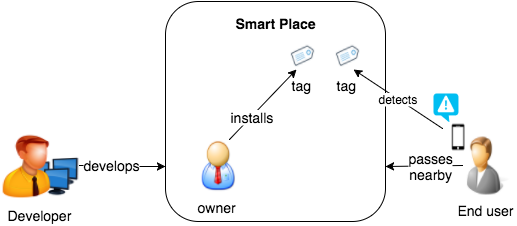
\includegraphics[width=0.8\textwidth, keepaspectratio]{images/smart_places_overview}
    \caption[Smart Places Overview]{Smart Places Overview}
    \label{fig:smart_places_overview}
\end{figure}

\section{Location}
\label{sec:background_location}
% Techniques
% Physical vs symbolic
% Absolute vs Relative
% Computed
% Scale
% Recognition
% Cost
% Limitations
In order to understand what a Smart Place is, we need to have a good insight about concepts related to location.
We have used a taxonomy\cite{location} to classify some properties about location.
These properties will allow us to have a better understanding about the concept of Smart Place, in section \ref{sec:background_smart_places}.
Also, these properties are needed to be able to classify the technologies, described in section \ref{sec:background_technologies} and justify if they can be used to implement the concept of Smart Place.
Using the taxonomy previously mentioned, it is possible to classify location systems in terms of techniques, physical position or symbolic location, absoulute or relative position, location computation, scale, recognition, cost and limitations.

\subsection{Techniques}
\label{sub:background_techniques}
There are three techniques that can be used to get the device's location.
These techniques are used to compute the location.
A device can use one or combine two or all the three.
Using one technique, does not mean that only that one can be used.
The techniques are the following:
\begin{description}
  \item[Triangulation] It can be done via lateration or angulation. Lateration uses distance measurements between two well known points.
  Angulation uses measurements of angles relative to known points;
  \item[Proximity] As the name suggests, it measures how close the device is to a known point;
  \item[Scene analysis] It consists in examining a view from a given point.
\end{description}

\subsection{Physical or Symbolic Position}
\label{sub:background_physical_or_symbolic_position}
The device's position can be classified in one of the two types:
\begin{description}
  \item[Physical position] This kind of position refers to a given set of coordinates that, identifies, unequivocally, a place on Earth where the device is. From this set of coordinates, we know, exactly, where the object is;
  \item[Symbolic location] Unlike physical location, using this kind of positioning, it is not possible to identify where the object is. Symbolic can be, for instance, the object is in the kitchen, office, etc. The meaning of its position depends on the application.
\end{description}

One location system can only be classified in one of the two kinds of positioning.
However, physical position can be augmented to also have symbolic information.
For instance, we can have a system that stores coordinates and for each set of coordinates we store symbolic information.
A place on Earth could have symbolic information associated.

\subsection{Computation}
\label{sub:background_computation}
We have multiple ways of obtaining data, about location and multiple kinds of location.
However, this data needs to be computed, somehow, in order to get meaning information about the object we want to locate.
This computation can be done in one of the two ways:
\begin{description}
  \item[Located object computes its own location] Here, the located object has means to compute its location itself;
  \item[Location is computed by external infrastructure] The located object delegates its location computation to an external infrastructure, for instance, a central server.
\end{description}

For instance, \gls{GPS} receivers compute their own location based on signals that come from satellites.
In location systems based on tags, the location's computation is delegated to another machine.

\subsection{Scale}
\label{sub:background_scale}
The scale of a location system refers to the number of objects that is possible to locate using a certain amount of infrastructure or over a given period of time.
For instance, in systems that rely on satelites with a fixed number of sattelites, it is possible to serve an unlimited number of receivers.
In systems based on tags, a reader can read a limited number of tags.
In this case, adding more tags can compromise the performance of the entire system.

\subsection{Recognition}
\label{sub:background_recognition}
Recognition refers to the hability, of a location system, to recognize individual receivers.
Location systems based on tags, usually, have means of recognizing receivers.
If we assign an \gls{ID} to each receiver, each time the receiver reads a tag, that information can be stored and it is possible to know which receiver communicated with that tag.
There are systems without this capability.
For instance, \gls{GPS} is a system that is not able to recognize receivers as the satelites do not have any means to recognize receivers.

\subsection{Cost}
\label{sub:background_cost}
There are costs associated to any location system.
It is possible to look at costs in three perspectives:
\begin{description}
  \item[Time costs] Any location system needs time to be spent in installation, administration and other tasks related with its maintenance;
  \item[Space costs] There is always some infrastructure associated with any location system. This infrastructure needs space. For instance, if servers are needed, we need to install them in some room;
  \item[Capital costs] The processes and infrastructure associated to a location system requires capital.
  Each mobile unit or infrastructure element has its price. Also, sometimes, there are people involved. Their salaries are also a capital cost that needs to be taken into consideration.
\end{description}

When comparing multiple location systems, the costs can be a decisive factor. We need not only to take into account the technology characteristics but also the costs.

\subsection{Limitations}
\label{sub:background_limitations}
There are no perfect location systems. Every system has its own limitations.
There are ones that do not work well indoors, such as, the \gls{GPS}, because it cannot get the sattelites' signal.
If we want a location system that would work indoors, maybe a tag based system is a better fit.
When choosing a system, this is important because one might not require much hardware and it leads to a low cost system but, if the limitations compromise its performance, it is better to pick one with higher costs.
For instance, a tag based system might only work properly if only one tag is present.

\section{Location Detection Technologies}
\label{sec:background_technologies}
% Possible technologies
% GPS
% QR Codes
% NFC
% Google maps indoor
% BLE
Before choosing a technology for tagging, we first need to relate Smart Places with the taxonomy introduced before.
They are based on the proximity technique and on symbolic location.
Also, we need to take into account the cost and limitations because we want a solution as low cost as possible, in terms of time and capital, for end users, owners and developers.

Somehow, the mobile device needs to be able to detect the presence of these tags.
Multiple technologies can be used.
Some of them require the user interaction, such as the described in section \ref{sub:background_qr_codes}.
Others require the devices to be equipped with extra hardware, such as the one in section \ref{sub:background_near_field _communication}.
We are going to look at these technologies and see which one best fits our purpose, using the taxonomy introduced in section \ref{sec:background_location}.

\subsection{\glstext{GPS}}
\label{sub:background_gps}
% What is it
% How it works
\glsfirst{GPS} is a location system that uses 24 sattelites plus 3 backups.
Receivers send signals and sattelites answer back. Measurements are taken from this signals in order to receivers be able to calculate their own location.
An object, that we want to locate, only needs a \gls{GPS} receiver in order to be located using this technology.

% Classification
\gls{GPS} uses triangulation as the technique to get the location.
It computes physical location, that is, when an object is located, we can look at a map and see where it is.
The located objects have means to compute their own location, based on measurements from the satellites' signals.
It is a scalable system because, the same number of satelites can handle an unlimited number of \gls{GPS} receivers.
The satelites are not able to recognize individual receivers.
In this system, the major cost is in maintaining the sattelites and, in the beginning, was launching the sattelites and, in the future, it might be necessary to replace the existing ones.
It cost 12 billion dollars to put them in orbit. The annual operating cost is 750 million dollars\footnote{Source: http://nation.time.com/2012/05/21/how-much-does-gps-cost at 24, December, 2015}.
One limitation of \gls{GPS} is that, it does not well indoors because the sattelite's signal can be really weak.

% Requirements
% Advantages and disadvantages
Objects to be located using \gls{GPS} only require an adequate receiver. Most of the mobile devices, nowadays, are already equipped with these receivers.
This can be a big advantage because it is a low cost solution for users.
However, as already mentioned, it is not adequate to locate objects indoors.

\subsection{QR Codes}
\label{sub:background_qr_codes}
% What is it
% How it works
\gls{QR} codes is a type of two dimensional barcode.
The user just needs a camera and software that read these codes.
There are \gls{QR} readers available for all the three major mobile platforms, Android, iOS and Windows Phone.
Whenever the user sees one of these codes, he/she can open the \gls{QR} code reader app, scan the code and see the content provided by it.
The content can be an \gls{URL}.
Figure~\ref{fig:qr_code} shows an example of a \gls{QR} code.

\begin{figure}[!ht]
  \centering
    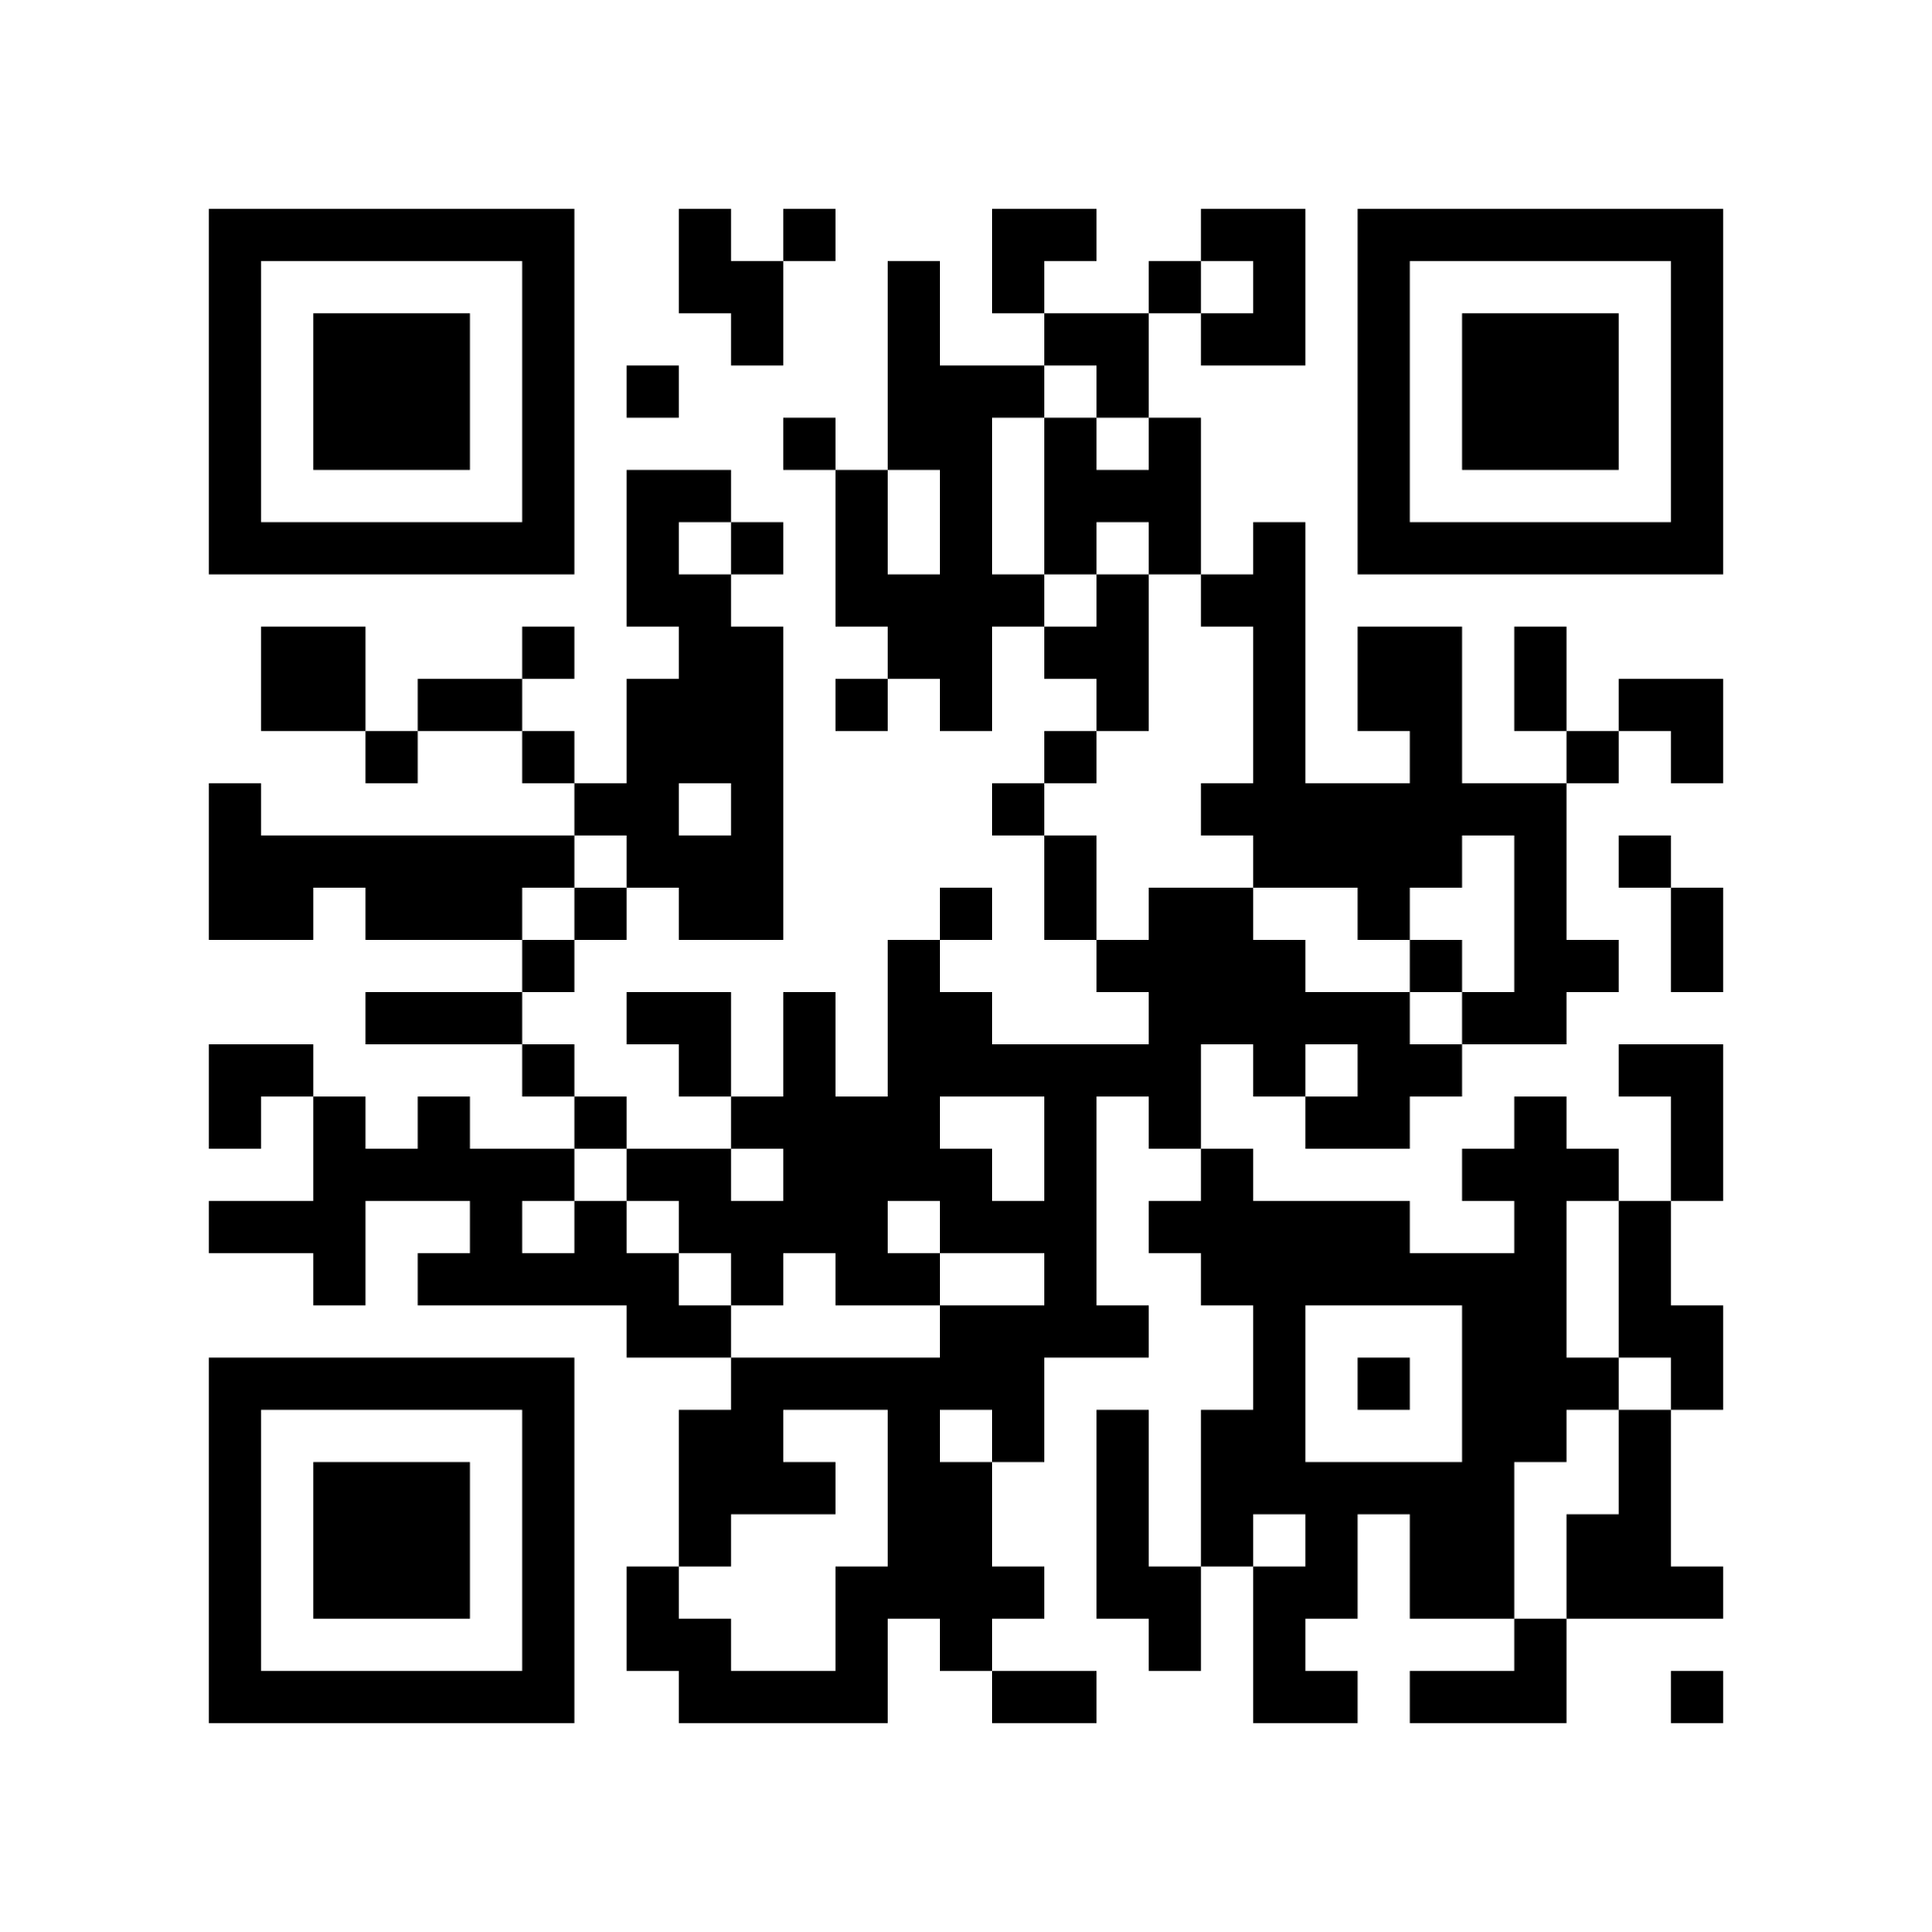
\includegraphics[width=0.3\textwidth, keepaspectratio]{images/qr_code}
    \caption{Example of a QR Code}
    \label{fig:qr_code}
\end{figure}

% Requirements
% Advantages and disadvantages
It does not require more than a mobile device with a camera and a \gls{QR} code reader app, such as, QR Droid\footnote{http://play.google.com/store/apps/details?id=la.droid.qr} for Android, QR Reader\footnote{http://itunes.apple.com/pt/app/qr-reader-for-iphone/id368494609?mt=8} for iOS and QR Code Reader\footnote{http://www.microsoft.com/en-us/store/apps/qr-code-reader/9wzdncrfj1s9} for Windows Phone.
There is no extra hardware involved.
However, one big disadvantage of this technology is the fact that it requires user interaction.
The user needs to be aware of this kind of codes and also needs to see them wherever they are.
Providing proximity-based services using \gls{QR} codes would be simply using the codes as tags and an app for users to scan these codes and have access to the particular service, that is, Smart Place.

% Related work
There are works that use this technology to to get the user's indoor location, such as, the one described in \cite{qr_indoor}.
It uses \gls{QR} codes in combination with \tm{Google} Maps \gls{API}\footnote{http://developers.google.com/maps}.
Others, try to use it to solve real world problems, such as, hospital overcrowding.
In the work, presented in \cite{qr_hospital}, the authors try to use \gls{QR} Codes to identify patients, in an hospital.
This information is used in a mobile application that the hospital's staff use to register activities related to the patient.

\subsection{NFC}
\label{sub:background_near_field _communication}
% What is it
% How it works
\glsfirst{NFC} is a short distance radio communication technology.
The two devices communicating need to be at 10 cm or less distant from each other.
Each \gls{NFC} device can work in one of three modes:
\begin{description}
  \item[Card Emulation] In this mode, devices act as if they were smart cards, allowing to perform transactions, such as payments;
  \item[Reader/Writer] Devices are enabled to read information from \gls{NFC} tags, embedded in other objects such as posters;
  \item[Peer-to-peer] Devices exchange information with each order in an adhoc way.
\end{description}

% Requirements
% Advantages and disadvantages
Simillary to \gls{QR} Codes, described in section \ref{sub:background_qr_codes}, this technology requires the user interaction and his/her awareness of the existence of these kinds of tags.
Also, devices need to be equipped with \gls{NFC} readers.
% Related work
This technology is already being used for payments, such as \tm{Apple} Pay\footnote{http://www.apple.com/apple-pay/}.

% Get references to this...
\subsection{Google Maps Indoor}
\label{sub:background_google_maps_indoor}
% What is it
% How it works
Google Maps allows users to navigate all over the world and gives access to satellite images.
There are mobile apps for Android and iOS.
With more than \num{1e9} installs on Google Play Store and an average rating of 4.3\footnote{Source: http://www.appannie.com/apps/google-play/app/com.google.android.apps.maps in 23 December 2015}, we can say it is a very popular and mainstream app.
When installed on a smartphone, it uses multiple sensors, such as, \gls{GPS} and accelerometer, in order to get the user's location.
However, since it relies on \gls{GPS}, it does not work well indoors.
Google Maps Indoor\footnote{http://www.google.com/maps/about/partners/indoormaps} is an extension which allows the user to navigate inside a building.
Figure~\ref{fig:google_maps_indoor} shows an example of Google Maps Indoor.

\begin{figure}[!ht]
  \centering
    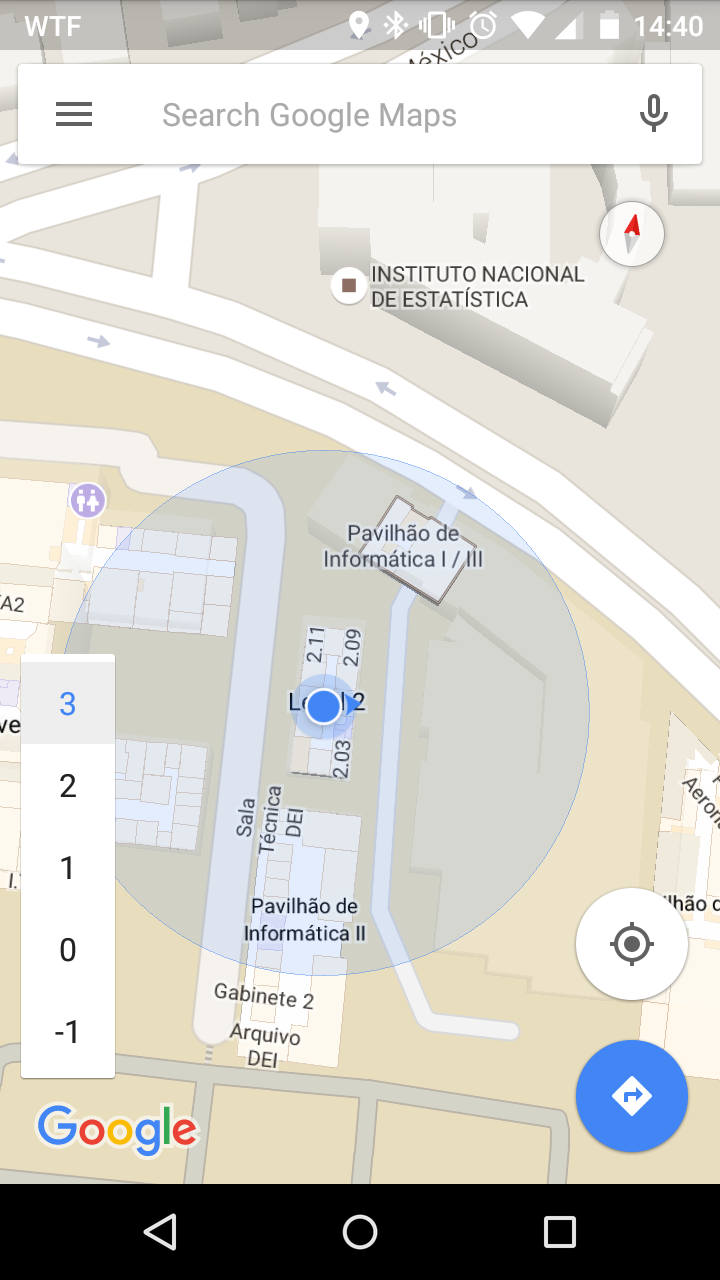
\includegraphics[width=0.3\textwidth, keepaspectratio]{images/screenshots/google_maps_indoor}
    \caption[Google Maps Indoor]{Screenshot of Google Maps with indoor functionality}
    \label{fig:google_maps_indoor}
\end{figure}

% Requirements
% Advantages and disadvantages
This service uses sensors already provided by the mobile device and it does not require extra sensors inside the building.

\subsection{Bluetooth Low Energy}
\label{sub:background_bluetooth_low_energy}
% What is it
% How it works
\glsfirst{BLE}\cite{ble} is a short range wireless communication technology, developed by Bluetooth \gls{SIG}\footnote{http://www.bluetooth.org}.
It is more focused on low power consumption than classic Bluetooth.
To take advantage of this technology, the mobile device needs to be equipped with Bluetooth, at least, version 4.0\cite{bluetooth_specification}.
However, to be able to use it, in order to get the user's indoor location, a protocol is needed.
There are two protocols that can be used: iBeacon\footnote{http://developer.apple.com/ibeacon}, developed by \tm{Apple} and Eddystone\footnote{http://github.com/google/eddystone}, developed by \tm{Google}.

% Protocols: ibeacon and eddystone
The iBeacon protocol works with small devices, named beacons, that broadcast a sequence of bytes, which acts as an identifier allowing to build proximity-based applications\cite{ibeacon_book}.
Figure~\ref{fig:ibeacon_message} shows the structure of this sequence of bytes, where it is possible to see three parts:
\begin{description}
  \item[\gls{UUID}] has 16 bytes (128 bits) and it identifies the organization that the beacon belongs to;
  \item[Major] has two bytes (16 bits) and it identifies a group of beacons that belong to a given organization identified by the \gls{UUID};
  \item[Minor] has two bytes (16 bits) and it identifies each individual beacon in the group identified bu the Major value.
\end{description}
In this protocol, location is reported to an application using one of the two operations:
\begin{description}
  \item[Monitoring] This operation is called when the beacon and the mobile device are in the same space;
  \item[Ranging] It is related to a single beacon. The distance from a mobile device to a beacon is estimated using its transmissions.
\end{description}

\begin{figure}[!ht]
  \centering
    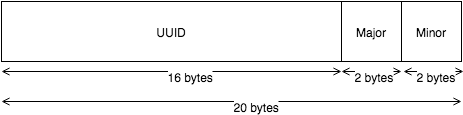
\includegraphics[width=0.6\textwidth, keepaspectratio]{images/ibeacon_message}
    \caption[iBeacon message structure]{Structure of the sequence of bytes transmitted in iBeacon protocol}
    \label{fig:ibeacon_message}
\end{figure}

In the other mentioned protocol, Eddystone the beacons also advertise a sequence of bytes.
However, there are three types of messages, that beacons can broadcast to mobile devices nearby\footnote{http://github.com/google/eddystone/blob/master/protocol-specification.md}:
\begin{description}
  \item[Eddystone-UID]
  It broadcasts an unique 16 byte (128 bits) identifier. The first 10 bytes are for the namespace, which is used to distinguish groups of beacons, and the remaining 6 are for the instance \gls{ID}, which is used to identify individual beacons, inside the same namespace;
  \item[Eddystone-URL]
  As the name suggests, it broadcasts an \gls{URL};
  \item[Eddystone-TLM]
  Here, telemetry information about the beacon is transmitted such as battery voltage and device's temperature.
\end{description}

% Requirements
% Advantages and disadvantages
The main advantage of this technology is that it only requires that the mobile device has Bluetooth 4.0.
However, to develop proximity-based applications, we need to deploy some beacons that use the iBeacon or the Eddystone protocol.
Fortunately, the extra hardware is the space owner's responsability.
The user does not need anything else besides his/her mobile device.

Using this technology, if developers want to map beacons to more kinds of information, only the mentioned protocols are not enough.
We need a backend to store the mapping between the beacons and that information.
Besides developing the application itself, developers also need to deal with the backend and all the concerns around any distributed system, such as, scalability, performance, etc.

\subsection{Overview}
\label{sub:background_overview}
% Main advantages of each one
% The chosen one (BLE ibeacon)
% Why
Multiple technologies were taken into consideration.
Ones are tag based, such as \gls{QR} codes, \gls{NFC} and \gls{BLE} that can be used to provide symbolic location.
Others, such as \gls{GPS} and Google Maps Indoor, are used to provide physical location but can be augmented to provide symbolic location.
However, \gls{GPS} does not work properly indoors and Google Maps Indoor requires that buildings are mapped first by a team from \tm{Google}.
Each technology was classified in terms of techniques, type of location (physical or symbolic), computation, scale, recognition of individual receivers, costs and limitations.
This classification was made using the taxonomy introduced in section \ref{sec:background_location} and is summarized in Table~\ref{tab:technologies}.

% Please add the following required packages to your document preamble:
% \usepackage{booktabs}
% \usepackage{graphicx}
\begin{table}[]
\centering
\resizebox{\textwidth}{!}{%
\begin{tabular}{@{}lllllll@{}}
\toprule
\textbf{Technology}                                                       & \textbf{Techniques} & \textbf{Type of location} & \textbf{Computation}                                                              & \textbf{Scale}                                                                        & \textbf{Costs}                                                               \\ \midrule
\textbf{GPS}                                                              & Triangulation       & Physical                  & In device                                                                         & \begin{tabular}[c]{@{}l@{}}24 satellites \\ serve unlimited \\ receivers\end{tabular} & Satellites                                                                   \\
\textbf{\begin{tabular}[c]{@{}l@{}}QR \\ Codes\end{tabular}}              & Proximity           & Symbolic                  & \begin{tabular}[c]{@{}l@{}}External \\ infrastructure\end{tabular}                & \begin{tabular}[c]{@{}l@{}}Depends on \\ the external \\ infrastructure\end{tabular}  & \begin{tabular}[c]{@{}l@{}}External\\ infrastructure\end{tabular}            \\
\textbf{NFC}                                                              & Proximity           & Symbolic                  & \begin{tabular}[c]{@{}l@{}}External \\ infrastructure\end{tabular}                & \begin{tabular}[c]{@{}l@{}}Depends on \\ the external \\ infrastructure\end{tabular}  & \begin{tabular}[c]{@{}l@{}}External\\ infrastructure\\ +\\ Tags\end{tabular} \\
\textbf{\begin{tabular}[c]{@{}l@{}}Google \\ Maps \\ Indoor\end{tabular}} & Triangulation       & Physical                  & \begin{tabular}[c]{@{}l@{}}In device\\ +\\ External\\ infrastructure\end{tabular} & \begin{tabular}[c]{@{}l@{}}Depends on\\ the external \\ infrastructure\end{tabular}   & \begin{tabular}[c]{@{}l@{}}External\\ infrastructure\end{tabular}            \\
\textbf{BLE}                                                              & Proximity           & Symbolic                  & \begin{tabular}[c]{@{}l@{}}External \\ infrastructure\end{tabular}                & \begin{tabular}[c]{@{}l@{}}Depends on \\ the external \\ infrastructure\end{tabular}  & \begin{tabular}[c]{@{}l@{}}External\\ infrastructure\\ +\\ Tags\end{tabular} \\ \bottomrule
\end{tabular}
}
\caption[Comparison of location technologies]{Comparison of location technologies}
\label{tab:technologies}
\end{table}


% Discussion of technologies
The concept of Smart Place is based on proximity and symbolic location.
Also, it is supposed to work indoors.
% GPS
\gls{GPS} is a location system that uses triangulation to provide physical location.
It is possible to augment physical location in order to provide symbolic.
However, it only works properly where it has a good receiption of the sattelites' signal.
Since the concept of Smart Place is a concept connected to an indoor space, the \gls{GPS} is not a good option, even if we augment it to provide symbolic location, because it does not work properly indoors.

% QR and NFC
\gls{QR} Codes and \gls{NFC} are based on the proximity technique.
They can provide symbolic location if enough data is stored in an external infrastructure.
The scale is dictated by this infrastructure and not not by the device that is being located.
The costs depend on the amount of infrastructure.
The main limitation of both is that it is only possible to read a tag at a time.
\gls{QR} Codes require that we spread codes which can be shown in a piece of paper.
\gls{NFC} tags are more expensive.
However, both would take us to a solution where the user interaction is required, that is, the user needs to be aware of existing tags and start the interaction instead of just being notified that a given proximity-based service is available at that location.
% Google Maps Indoor
Smart Places could be implemented using Google Maps Indoor.
This technology is based on triangulation technique and provides physical location.
Similar to \gls{GPS} it can be augmented to provide symbolic location requiring a given amount of external structure, which is what scale depends on and the major cost here.
This would lead to a solution where no extra hardware is needed.
However, it requires that a team from \tm{Google} maps the building first in order to be possible to navigate in it using Google Maps Indoor.
% BLE
\gls{BLE} is a good fit for our purpose because, it is based on proximity and can be used to provide symbolic location.
It does not have any costs for the users besides the acquisition of the mobile device.
We can place the beacons wherever we want and where it makes sense for the service we want to provide.
Also, using this technology, the mobile app that will handle the nearby beacons, can be running in background.
This way, the user does not to be aware of any tags and he/she can be notified if a proximity-based service is found.

% Final decision -> BLE
The final decision was to pick \gls{BLE} because it has the best tradeoff between cost and kind of location it provides. Using this technology we have symbolic location. With the adequated infrastructure it is possible to associate any kind of information to each tag.
It requires extra hardware but this is the responsability of who manages the place where the tags will be deployed.
The user does not need anything else but a mobile device with Bluetooth, version 4.0 or later.
Three beacons, from \tm{Estimote} were used in the implementation of our solution, described in chapter \ref{chapter:implementation}.

\section{Summary}
\label{sec:background_summary}
% Location
% -> Introduced taxonomy (techniques, physical vs sumbolic, computation, scale, recognition, cost and limitations)
In the previous chapter, we introduced the problem that this work tries to solve.
However, before describing the solution, we need first to understand some concepts.
In this chapter we introduced a taxonomy to classify location systems, in terms of techniques, physical or symbolic location, computation, scale, recognition, cost and limitations.
There are three types of techniques: Triangulation, proximity and scene analysis.
Triangulation is based on measures, distance or angles, between two well known points, proximity takes into account the distance to a given point and scene analysis is based on an analysis of a view from a given point.
The location can be physical, which refers to identifying where, exactly, the object is. In symbolic location, it is not possible to identify where the object is. Instead, its location depends on the context.
Location information can be computed by the located object itself or by an external infrastructure.
The scale of a location system refers to how many objects is possible to locate with a given amount of infrastructure or over a period of time.
Recognition refers to if it is possible to recognize individual receivers.
There are three main types of costs.
Time costs represent the time needed for tasks, such as, installation or administration.
Space costs are related to the area needed for the necessary infrastructure. Capital costs refer to the capital needed to install and maintain a location system.
Also, there is no best location system. Each one has its own limitations.

% Smart Place (based on taxonomy)
The concept of Smart Place was defined as a place, with tags, that provide a service, to users, when they approach those tags.
Using the taxonomy, introduced before, in order to support this concept, we need a location system that is based on the proximity technique and provides symbolic location.
A Smart Place involves three groups of people: Owners, who are responsible for managing a Smart Place, developers, who develop proximity-based services and end users who are, anyone, with a mobile device, capable of detecting tags.

% Technologies
% -> GPS, QR Codes, NFC, GMI, BLE
% -> Chose BLE because...
In our solution, we need to choose a location system.
We analyzed several technologies, such as, \gls{GPS}, \gls{QR} Codes, \gls{NFC}, Google Maps Indoor and \gls{BLE}, according to the taxonomy introduced before.
We concluded that the \gls{BLE} using ibeacon protocol is the best option, because, it works well indoors, unlike \gls{GPS}.
Also, it does not require user interaction, as it is in \gls{QR} Codes or \gls{NFC}.
Using this technology, owners can place tags anywhere, without the need to, first, mapping the entire area, as it is needed in Google Maps Indoor.
